\subsection{Simple linear regression}

Various aspects of the standard data ellipse of radius 1 illuminate many properties
of simple linear regression, as shown in \figref{fig:ellipses-demo}.
These properties are also useful in more complex contexts.

\begin{figure}[htb]
  \centering
  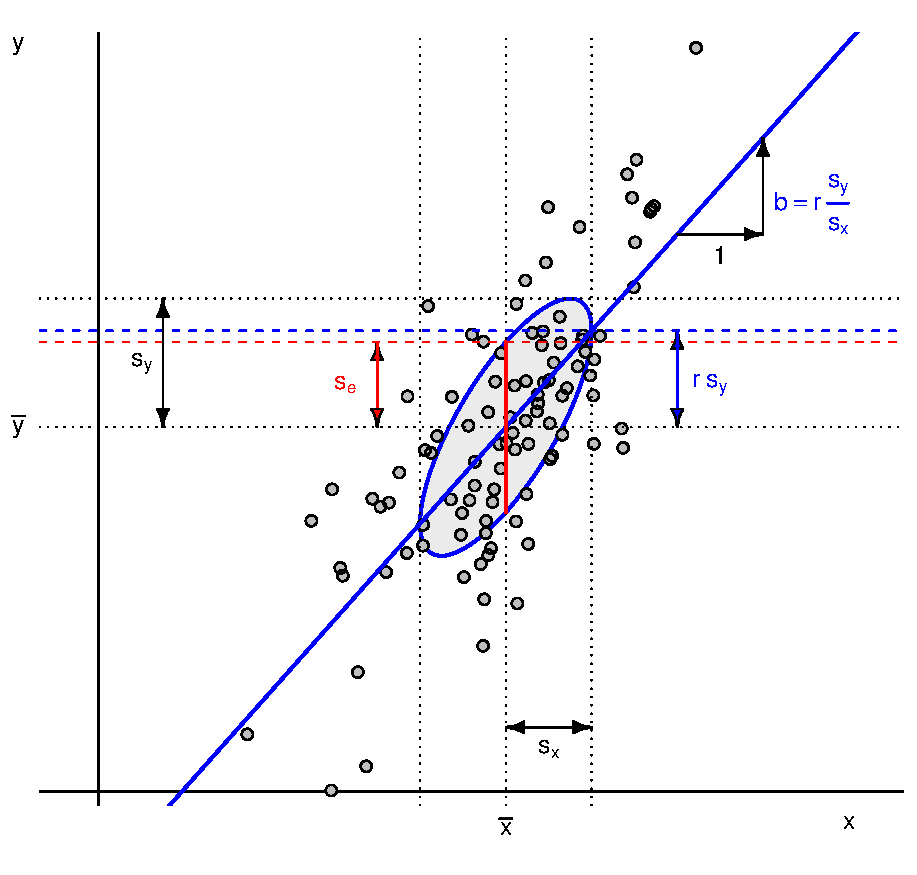
\includegraphics[width=.6\textwidth,clip]{fig/ellipses-demo}
  \caption{Annotated standard data ellipse showing standard deviations of $x$ and $y$, residual
  standard deviation ($s_e$), slope ($b$), and correlation ($r$).
  }%
  \label{fig:ellipses-demo}
\end{figure}

\begin{itemize}
  \item One-half of the widths of the vertical and horizontal projections (dotted black lines)
  give the standard deviations $s_x$ and $s_y$ respectively.
  \item Because the perpendicular projection onto any line through the center of the ellipse ($\bar{x}, \bar{y}$), corresponds to
  some linear combination, $m x + n y$, the half-width of the corresponding projection of the ellipse
  gives the standard deviation of this linear combination.
  \item With a multivariate normal distribution the line segment through the center of the ellipse
  shows the mean and standard deviation of the conditional distribution on that line.
  \item The standard deviation of the residuals, $s_e$ can be visualized as the half-width of the vertical
  (red) line at $x=\bar{x}$.
  \item The vertical distance between the mean of $y$ and the points where the ellipse has vertical
  tangents is $r s_y$. (As a fraction of $s_y$, this distance is $r = 0.75$ in the figure.)
  \item The (blue) regression line of $y$ on $x$ passes through the points of vertical tangency.
  Similarly, the regression of $x$ on $y$ (not shown) passes through the points of
  horizontal tangency.

\end{itemize}

\subsection{Visualizing a confidence interval for the slope}

A visual approximation to a 95\% confidence interval for the slope, and thus a visual test of $H_0: \beta = 0$
can be seen in \figref{vis-reg-prestige}.  From the formula for a 95\% confidence interval,
$\mathrm{CI}_{.95} (\beta) = b \pm t_{n-2}^{0.975} \times \mathrm{SE}(b)$, we can take $t_{n-2}^{0.975} \approx 2$
and
$\mathrm{SE}(b) \approx \frac{1}{\sqrt{n}}\left( \frac{s_e}{s_x} \right)$,
leading to
\begin{equation}\label{eq:ci-approx}
\mathrm{CI}_{.95} (\beta) \approx b \pm \frac{2}{\sqrt{n}} \times \left( \frac{s_e}{s_x} \right) \period
\end{equation}
%\todo{fix the notation in these figures}
\begin{figure}[htb]
% two figs side-by-side
  \begin{minipage}[c]{.49\textwidth}
   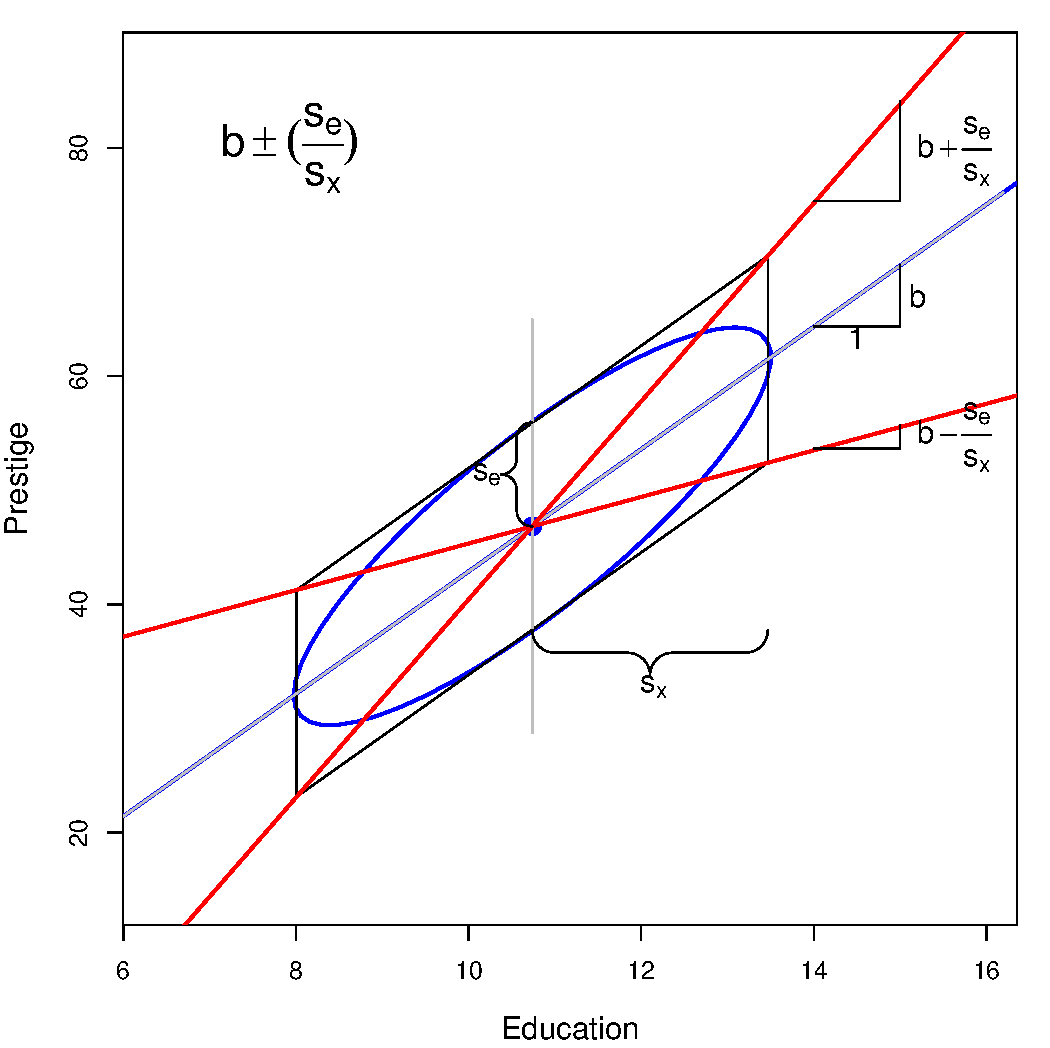
\includegraphics[width=1\linewidth,clip]{fig/vis-reg-prestige1}
   \end{minipage}%
  \hfill
  \begin{minipage}[c]{.49\textwidth}
   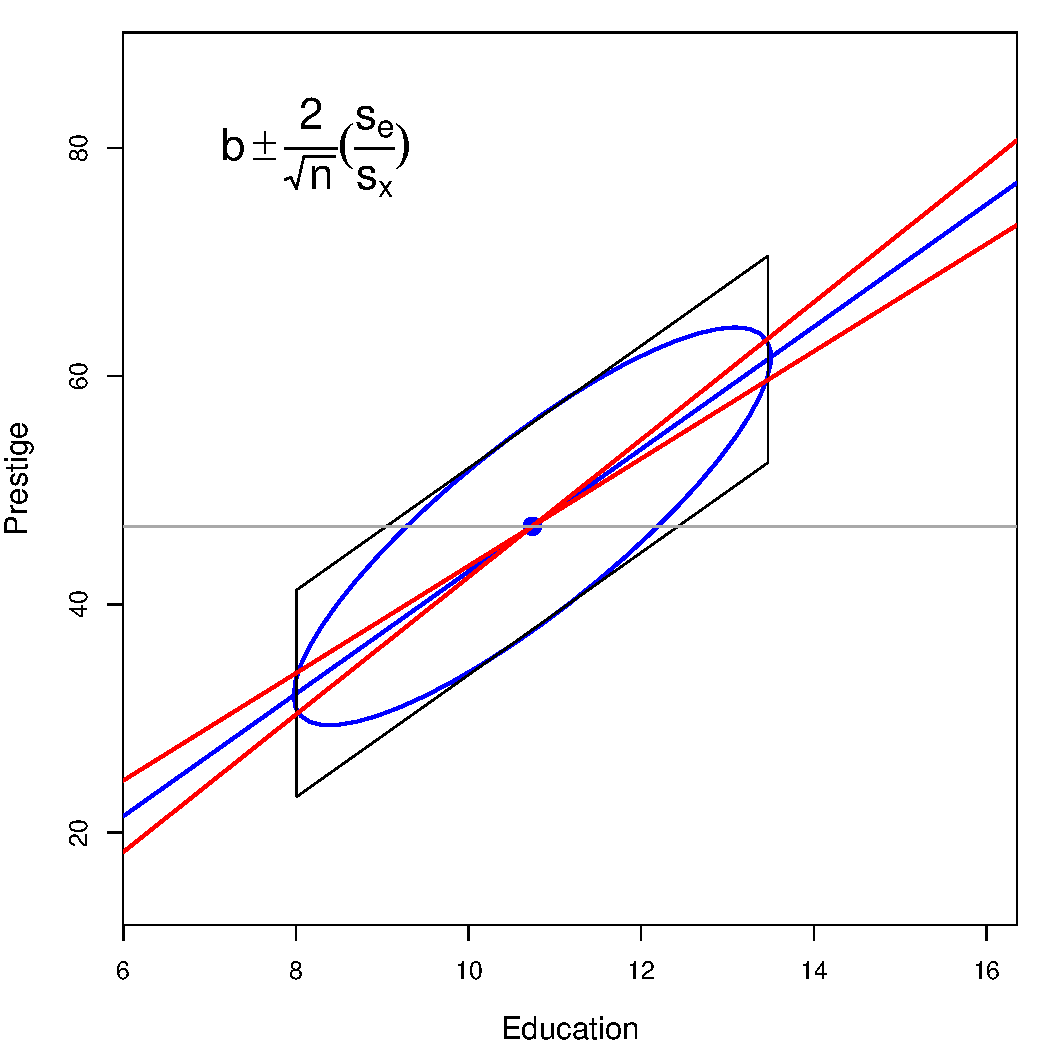
\includegraphics[width=1\linewidth,clip]{fig/vis-reg-prestige2}
  \end{minipage}
  \caption{Visual 95\% confidence interval for the slope in linear regression. Left: Standard data ellipse surrounded by the
  regression parallelogram. Right: Shrinking the diagonal lines by a factor of $2/\sqrt{n}$,
  gives the approximate 95\% confidence interval for $\beta$.}%
  \label{vis-reg-prestige}
\end{figure}

To show this visually, the left panel of \figref{vis-reg-prestige} displays the standard data ellipse
surrounded by the ``regression parallelogram,'' formed with the vertical tangent lines and the
tangent lines parallel to the regression line. This corresponds to the conjugate axes of the
ellipse induced by the Choleski factor of $S_{yx}$ as shown in \figref{fig:conjugate} in \appref{sec:conjugate}.
Simple algebra demonstrates that the diagonal lines through
this parallelogram have slopes of
\begin{equation*}
 b \pm \frac{s_{e}}{s_x}
\end{equation*}
So, to obtain a visual estimate of the 95\% confidence interval for $\beta$ (\emph{not}, we note, the 95\% CI for the regression line), we need only shrink the diagonal lines of the
regression parallelogram toward the regression line by a factor of $2/\sqrt{n}$, giving the red lines
in the right panel of \figref{vis-reg-prestige}.
In the data used for this
example, $n=102$, so the factor  is approximately 0.2 here.\footnote{The data are for the rated prestige and average years of education of 102 Canadian occupations circa 1970; see \citet{FoxSuschnigg:89}.}
Now consider the horizontal line through the center of the data ellipse.  If this line is outside the
envelope of the confidence lines, as it is in \figref{vis-reg-prestige}, we can reject $H_0: \beta = 0$ via this simple visual approximation.
